\section{Visão global do jogo}

Neste capítulo é apresentado as características principais do jogo. 
Alem disso são descritas as referencias usadas para o desenvolvimento 
e criação do mesmo. 

\subsection{Enredo}
Medrash, um jovem caçador da pequena e pacífica tribo Ari, ao retornar de
 uma caçada na noite anterior, encontra sua tribo completamente devastada 
na manhã seguinte. Nela, há apenas um sobrevivente dentre os feridos
 agonizantes, seu amigo Gardain, um dos mais fortes guerreiros locais, que
 mesmo gravemente machucado, consegue contar à Medrash que na noite anterior
 eles foram surpreendidos por guerreiros da poderosa tribo Luskan - a mais
 temida dentre todas da região - e que não tiveram chance de se defender 
do ataque. Os sobreviventes de sua tribo foram levados pelos luskans para
 serem escravizados. Este ataque havia sido orquestrado por seu 
arqui-inimigo, Balasar, líder da tribo inimiga. Como se não bastasse a
 tragédia ocorrida, Medrash ainda é informado que os luskans haviam levado
 dentre os prisioneiros sua amada esposa, Sora.  Desesperado, Medrash 
inicia uma jornada contra o tempo em direção aos inimigos, rastreando 
a trilha deixada por eles. 

Ao final da trilha, após lutar contra as mais diversas adversidades e
 perigos, Medrash finalmente alcança seus inimigos; entretanto, antes que
 pudesse tomar qualquer atitude, ele  surpreende-se com o que presencia
 diante de seus próprios olhos: os aliados, da tribo Mara-kai, estão sob
 pesado ataque dos luskans, estratégia semelhante ao que havia ocorrido 
com sua tribo natal anteriormente. Após o cessar fogo e retirada inimiga,
 a devastação e o caos são eminentes entre as dependências dos mara-kais. 
Em sua busca por sobreviventes, Medrash encontra Rangrim, líder da tribo
 aliada ferido, que lhe dá a terrível notícia de que os inimigos marcham
 agora rumo à Akanul - a última e mais importante das tribos aliadas 
locais. Como já não haviam mais guerreiros das tribos atacadas que
 poderiam ajudar Medrash em um contra-ataque para libertar os membros
 capturados, a única alternativa agora seria chegar à Akanul antes dela 
ser destruída pelos luskans. Para isto, Rangrim indica um atalho pelas
 montanhas frias e selvagens Kabalus.
 
Felizmente, após a difícil e perigosa jornada pelas montanhas, Medrash 
chega a tempo de informar à tribo da invasão que eles sofreriam. Preparados,
 os akanuls conseguem se defender e evitam que seus membros sejam levados
 para a escravidão. Em busca de resgatar seus amigos e sua querida amada, 
Medrash e os demais guerreiros partem em direção à Luskan. Após vários
 confrontos com os inimigos, Medrash e os demais aliados 
conseguem libertar os escravos; contudo, sua amada não encontrava-se junto 
a eles: Sora estava com o temido Balasar. Para resgatá-la, Medrash terá que
 enfrentar seu algoz sozinho em uma batalha corpo-a-corpo de vida ou morte.

\subsection{Características gerais}
Abaixo apresentamos as principais características gerais do jogo:
\begin{itemize}
\item {\bf Estilo}
Ação/Aventura. 
\item{\bf Perspectiva}
Câmera fixa atrás do personagem.
\item{\bf Modo}
Mono Jogador.
\item{\bf Número de fases}
Três Fases.
\item{ \bf Linha do tempo}
Pré-Histórico 
\item{ \bf Idioma do jogo}
Português
\item{ \bf Plataforma}
\textit{Windows}
\item{\bf Gráficos}
3D
\item{ \bf Principal Forma de Controle}
Uso de teclado do computador.
\end{itemize}

\subsubsection{Descrição do jogo}
As Crônicas de Medrash apresenta um jogo caracterizado como \textit{Adventure},
 onde o personagem principal, Medrash, tem sua tribo devastada por seu inimigo 
Balasar e precisa correr contra o tempo para resgatar seus amigos e 
principalmente sua esposa Sora.
Nesta longa jornada, nosso herói Medrash enfrentará os perigos da floresta: 
animais perigosos, adversidades climáticas, aliados de Balasar e a si mesmo, 
superando fome e cansaço.
O jogo se passa em um ambiente hostil de floresta, envolvendo o jogador com a 
trama. Serão apresentadas duas fases durante o dia (sendo estas a primeira e terceira)
 e a segunda durante a noite - nesta apresentando-se sombria e com uma visão 
mais limitada do personagem. Ao final de cada fase o jogador vai se deparar com 
um desafio mais perigoso, popularmente conhecido como ``Chefe de fase'', necessitando 
de mais habilidades e recursos para alcançar a vitória.

\subsubsection{Motivação}

O jogo ``As Crônicas de Medrash'' será desenvolvido como trabalho para
 a disciplina IA369 do primeiro semestre de 2012, cujo objetivo é um exercício 
prático do projeto de um jogo digital, cobrindo todas suas etapas, que envolvem 
aspectos gerenciais, artísticos e técnicos associados ao desenvolvimento do mesmo.
A idéia das ``Crônicas de Medrash'' surgiu de comum acordo entre os membros
 do grupo, sendo um reflexo dos gostos e interesses compartilhados. A proposta 
é fazer um jogo que cumpra todas as características desejadas pelos integrantes 
do grupo, para isso foram formadas quatro equipes que desenvolvem atividades 
especificas na criação do jogo, o qual tem permitido que o processo de criação e 
desenvolvimento do jogo seja amigável para todos os integrantes, conseguindo 
a motivação de trabalho em equipe para conseguir um objetivo em comum para todos.

\subsubsection{Ambientes a serem simulados}
Serão simulados três ambientes no decorrer do jogo:

\begin{itemize}
\item Primeira fase: 
O primeiro cenário representa uma floresta de coníferas, a qual esta dividida em 
4 regiões. Na região ``A'' encontra-se a tribo ``ARI'', a qual localiza-se na parte mais alta
 da floresta numa montanha, este o ponto de inicio do jogo. Para deslocar-se entre
 as regiões ``A'' e ``B'', o personagem deverá descer a montanha pulando entre pedras.
 A região ``A'' estará infestada por cobras. A região ``B'' é composta por muitas árvores,
 esta região será dominada por ursos alem que ter enxames de abelhas. Na região ``C'' 
existe um rio com jacarés e finalmente na região ``D'' encontra-se o inimigo final da fase 1 
que é o tigre.

\item Segunda fase: 
A segunda fase é desenvolvida na noite em sua totalidade, a região toda está infestada 
por lobos. O personagem principal tem uma tocha acesa, que deverá ser mantida durante a fase.
 O cenário está coberto de neve, e o percurso tem muitos buracos que incrementam 
a dificuldade da fase. No final da fase o personagem tem que defender uma moradia 
da tribo aliada que está sendo atacada.

\item Terceira fase: 
A terceira fase é a fase final do jogo e possuí um clima de guerra total,
 onde o personagem principal tem que salvar Sora, sua esposa. Este cenário tem 
um vulcão que acrescenta um desafio para finalizar o jogo. 
\end{itemize}


\subsubsection{Personagem controlado pelo jogador}
O jogador controla o Medrash (personagem principal do jogo), que é um 
homem primata na casa dos 20 anos. Medrash tem os movimentos de correr, pular, 
pegar e bater no inimigo. Estas habilidades são usadas durante todo o percurso do jogo. 
O personagem principal é descrito em detalhes no Capítulo 3.

\subsubsection{Personagem controlado pelo computador}
Em cada uma das fases do jogo existem personagens controlados pelo computador, que 
são detalhados a seguir:


\subsubsection{Animais}
Estes se apresentam nas fases 1 e 2.
Fase1: Cobras, ursos, enxames de abelhas, jacarés e tigre (Chefe 1).
Fase2: lobos
Os animas se encontram durante as duas primeiras fases oferecendo desafio a Medrash. 

\subsubsection{Guerreiros}
Estes inimigos se apresentam nas fases 2 e 3. Os guerreiros, assim como os animais, 
tem a finalidade de oferecer desafio a Medrash. Cada guerreiro é membro de uma tribo, 
que pode ser Ari, Mara-Kai, Akanul ou Luskan. Somente os membros da tribo Luskan atacam 
Medrash, por ser a única tribo inimiga. 

\subsubsection{Principal objetivo do jogo}
O objetivo principal do jogo consiste em Medrash (personagem principal) resgatar 
sua tribo e a sua mulher, Sora. Tanto Sora como os membros de sua tribo 
estão presos na tribo Luskan, que tem como chefe Balasar, o inimigo principal de Medrash. 

\subsection{Referências e inspirações}
Nesta seção são listados alguns jogos que serviram de referência e inspiração 
para o desenvolvimento do jogo ``As Crônicas de Medrash''.

\begin{itemize}
\item {\bf Crash Bandicoot\cite{bib:crash_game}}
O jogo consiste 
em uma série de fases de aventura, inicialmente desenvolvido pela Naughty Dog.
Este jogo apresenta ambientes de movimentação de personagem limitados, ou seja, 
o personagem não pode se movimentar livremente para qualquer espaço que desejar.
 Desta forma o jogador é orientado a seguir um caminho e enfrentar os desafios 
oferecidos por obstáculos, tais como buracos e blocos de pedras, e inimigos.
Os inimigos são derrotados saltando-se sobre eles ou apenas encostando caso o jogador tenha pego a fruta ``Wunpa''.
No terceiro jogo desta série há a questão do tempo, pois se o jogador concluir a fase
 dentro de um tempo estipulado ganhará objetos que serão úteis no decorrer do jogo. A figura \ref{img:crash} mostra imagens deste jogo.

\begin{figure}[!ht]
 \centering
 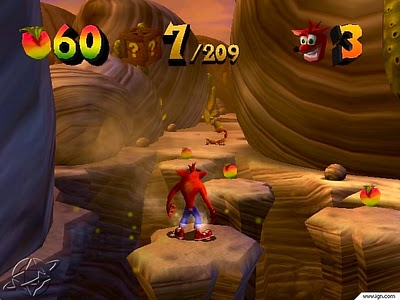
\includegraphics[scale=0.705]{Imagens/crash1.png}
 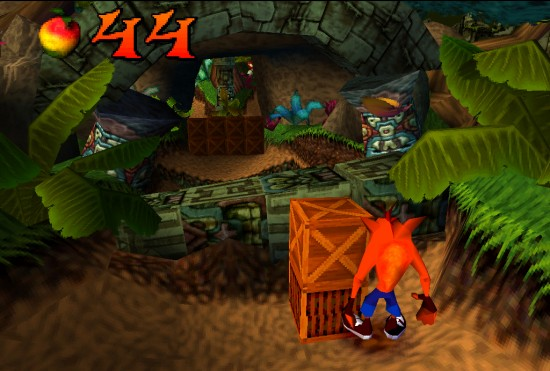
\includegraphics[scale=0.57]{Imagens/crash2.png}
 \caption{Captura de tela do jogo \textit{Crash Bandicoot}
(Fonte: \cite{bib:crash01,bib:crash02})}
 \label{img:crash}
\end{figure}

\item {\bf Super Mario Galaxy\cite{bib:mario_game}}
O jogo \textit{Super Mario Galaxy} é um jogo de aventura 3D produzido 
pela Nintendo EAD Tóquio. A ação se passa 
em terceira pessoa e o jogador deve controlar o personagem em uma aventura 
galáctica para salvar a princesa Peach.
Este jogo, eleito o melhor jogo da história da Nintendo, conta com diversos 
efeitos gravitacionais que proporcionam uma jogabilidade diferenciada, assim como 
é demonstrado na figura \ref{img:mario}. É importante ressaltar que como o jogo acontece no 
espaço, cada planeta tem suas características próprias, como por exemplo, 
gravidades diferentes. 
Esta jogabilidade permite jogos de câmeras não convencionais, movimentando a
 mesma de acordo com a posição do jogador e também do ``corpo celeste'' em que
 este se encontra.
Nas imagens abaixo é possível observar capturas de tela do \textit{Super Mario Galaxy}.

\begin{figure}[!ht]
 \centering
 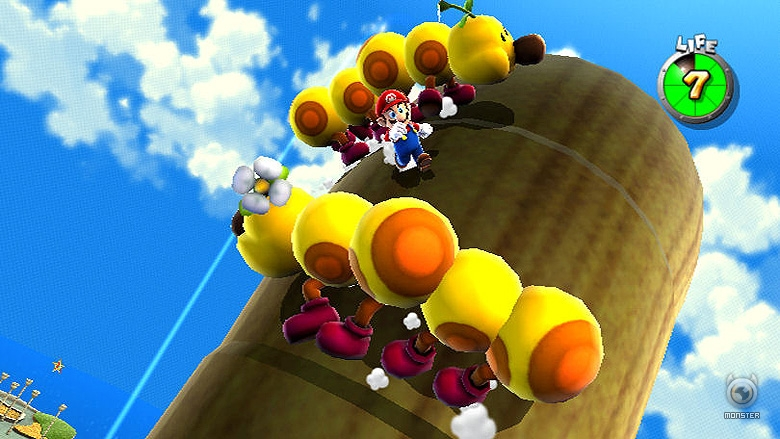
\includegraphics[scale=0.4]{Imagens/mario1.png}
 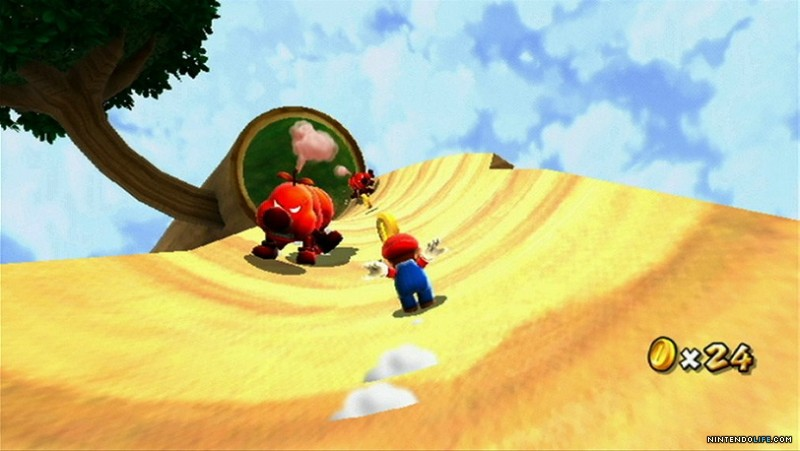
\includegraphics[scale=0.4]{Imagens/mario2.png}
 \caption{Captura de tela do jogo \textit{Super Mário Galaxy}
(Fonte: \cite{bib:mario01,bib:mario02})}
 \label{img:mario}
\end{figure}

\item {\bf Zelda\cite{bib:zelda_game}}
Dos jogos utilizados como referência para o desenvolvimento de
 ``As Crônicas de Medrash'',
\textit{Zelda} é o que conta com a maior liberdade de movimentação, embora ainda conte com 
caminhos específicos e ações determinadas a serem seguidas.
Neste jogo ocorre uma mistura a partir de uma trama complexa utilizando 
elementos de jogos de aventura com elementos de jogos de estratégia, os \textit{RPG}. 
Esta mistura de gêneros faz com que \textit{Zelda} se destaque com sua jogabilidade e
 possibilidades de exploração. 
A série \textit{Zelda} apresenta algumas características inovadoras. Em um dos jogos
 da série \textit{Zelda}, o \textit{Ocarina of Time}, o jogador utiliza-se de mira fixa, uma diferença 
com relação ao Mário 64, por exemplo.
Na Figura \ref{img:zelda} constam exemplos da ação no jogo \textit{Zelda}.

\begin{figure}[!ht]
 \centering
 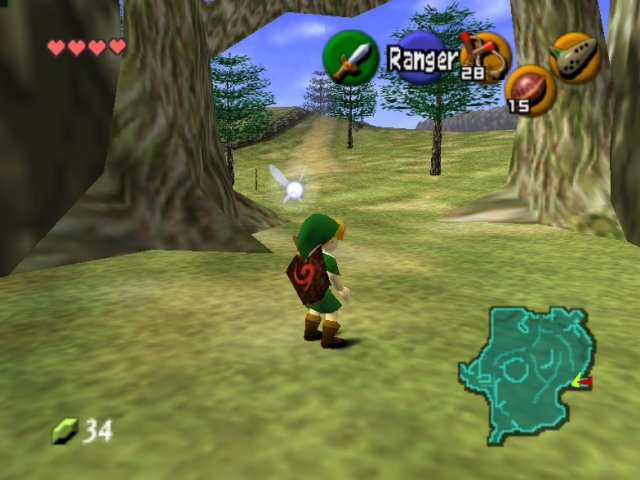
\includegraphics[scale=0.35]{Imagens/zelda1.png}
 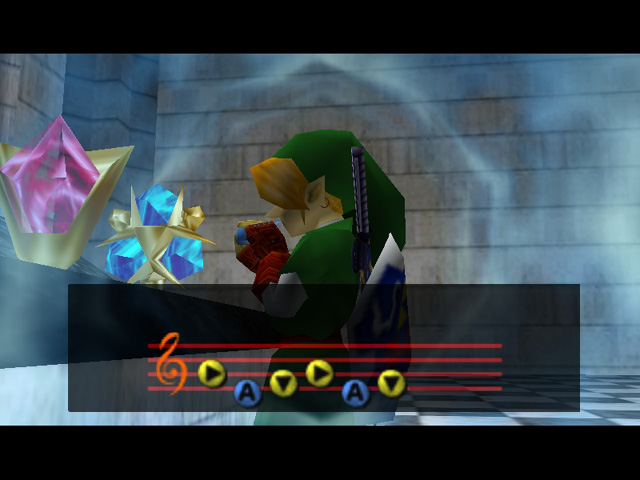
\includegraphics[scale=0.35]{Imagens/zelda2.png}
 \caption{Captura de tela do jogo \textit{Legend of Zelda}
(Fonte: \cite{bib:zelda01})}
 \label{img:zelda}
\end{figure}

\item {\bf Pitfall 3D\cite{bib:pitfall_game}}
\textit{Pitfall 3D}
 é um jogo onde o desafio é manipular o personagem através de uma floresta 
que se dispõe como um tipo de labirinto. Para vencer o jogador deve recolher 
tesouros em um determinado espaço de tempo vencendo desafios (poço de piche, 
areia movediça, buracos, troncos de árvore rolando, cascavel, escorpião, fogo, 
morcego e crocodilo).
O jogo ``As Crônicas de Medrash'' se desenvolve de maneira parecida, exigindo 
além da orientação do personagem pelo mapa a coleta de itens como alimento e fogo.

\begin{figure}[!ht]
 \centering
 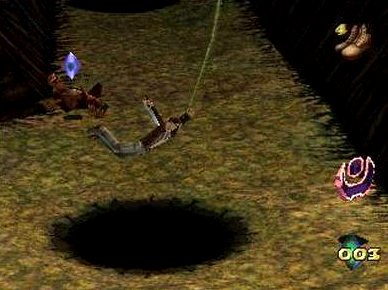
\includegraphics[scale=0.62]{Imagens/pit1.png}
 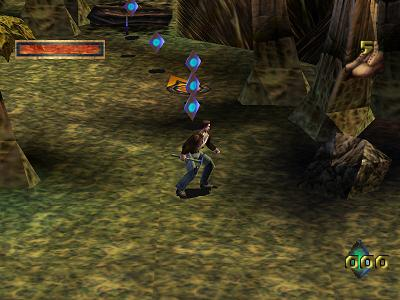
\includegraphics[scale=0.6]{Imagens/pit2.png}
 \caption{Captura de tela do jogo \textit{Pitfall 3D}}
 \label{img:pitfall}
\end{figure}

\end{itemize}